\documentclass{article}
\usepackage[margin=1in]{geometry}
\usepackage{graphicx}
\usepackage{listings}
\usepackage[utf8]{inputenc}
\usepackage{textcomp}
\usepackage{xcolor}
\definecolor{codegreen}{rgb}{0,0.6,0}
\definecolor{codegray}{rgb}{0.5,0.5,0.5}
\definecolor{codepurple}{rgb}{0.58,0,0.82}
\definecolor{backcolour}{rgb}{0.95,0.95,0.92}
\graphicspath{ {../src/assets/} }
\title{COMP 353 Main Project (iyc353\_1)}
\author{Luigi Besani Urena (40030054) \and Anoop Pukulakatt (40130695) \and Abdul Sirawan (40074202)
    \and Jeffrey Wilgus (29206345)}
\date{August 9, 2020}
\lstset{
    backgroundcolor=\color{backcolour},   
    commentstyle=\color{codegreen},
    keywordstyle=\color{magenta},
    numberstyle=\tiny\color{codegray},
    stringstyle=\color{codepurple},
    basicstyle=\ttfamily\tiny,
    breakatwhitespace=false,         
    breaklines=true,                 
    captionpos=b,                    
    keepspaces=true,
    language=SQL,
    literate={é}{{\'e}}1,
    showspaces=false,                
    showstringspaces=false,
    showtabs=false,                  
    tabsize=2,
    upquote=true
}
\newcommand{\tdash}{\textnormal{-}}
\begin{document}
    \maketitle
    \thispagestyle{empty}
    \newpage
    \clearpage
    \pagenumbering{arabic}
    \section{Design}
        \par Figure \ref{fig:erd} shows the entity-relationship diagram for the Web Career Portal database, and Figure
        \ref{fig:schema} shows the derived database schema. \par
        \begin{figure}[h]
            \centering
            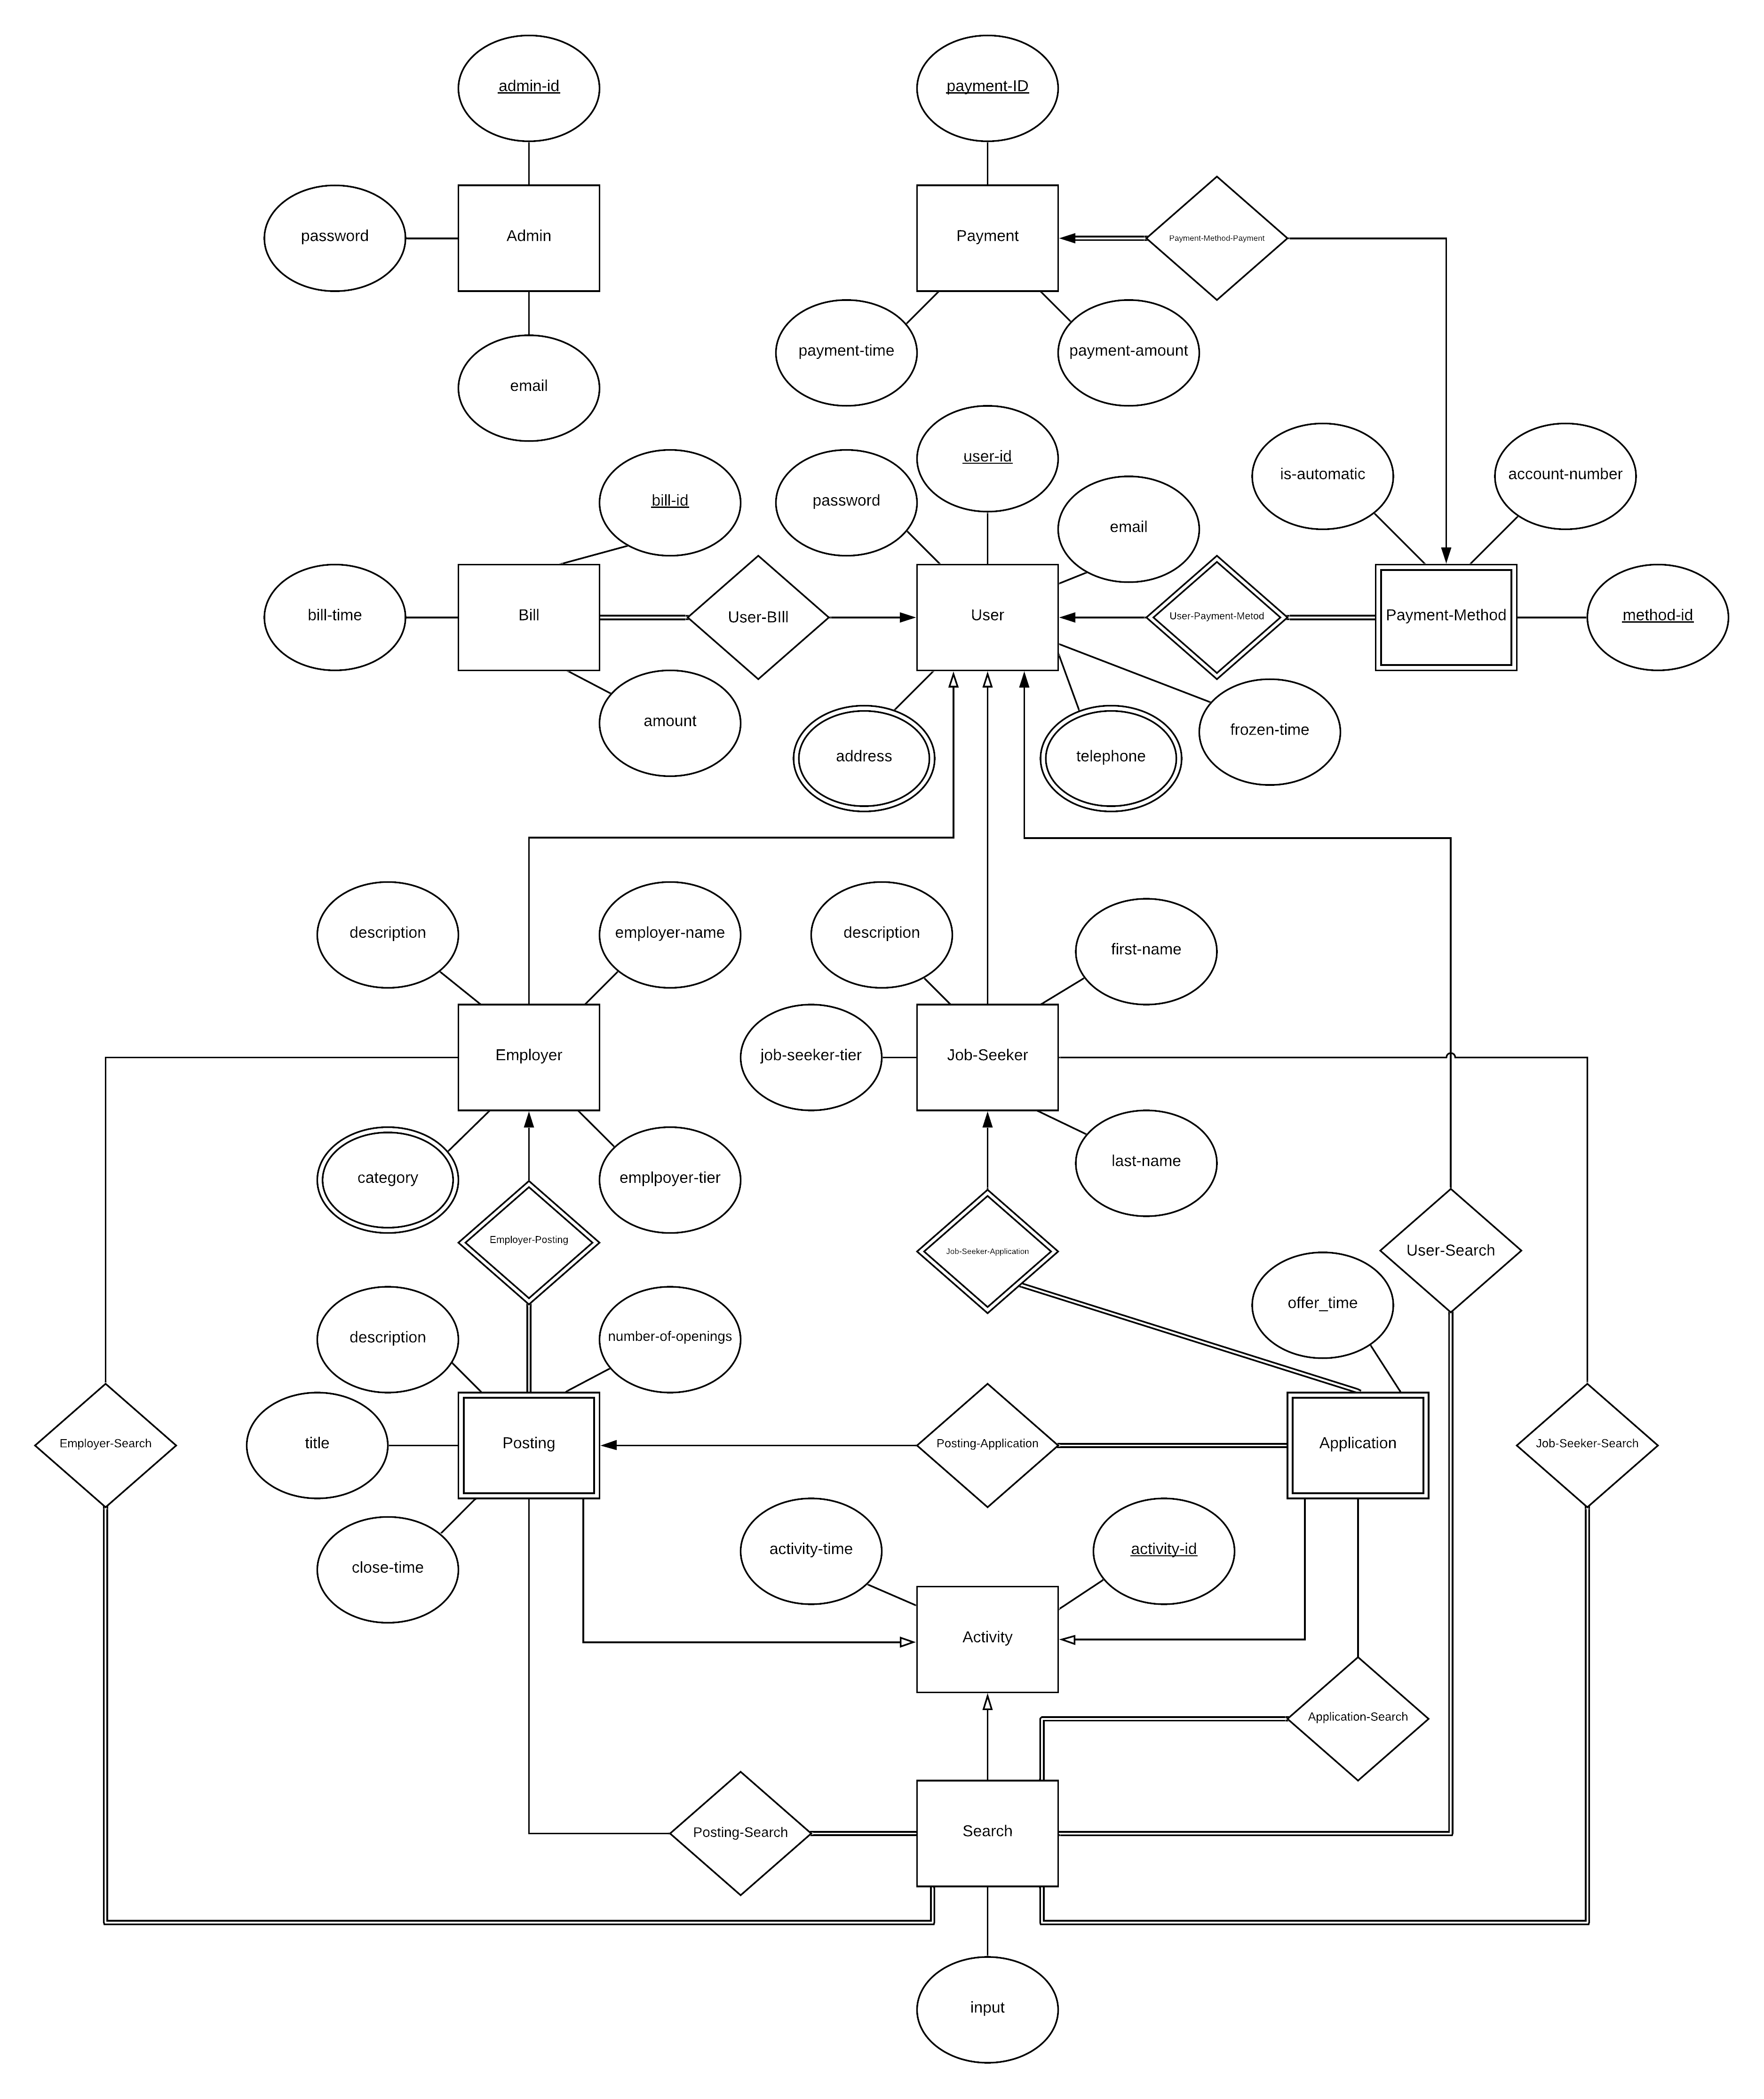
\includegraphics[scale=0.1]{erd}
            \caption{Web Career Portal ER Diagram}
            \label{fig:erd}
        \end{figure}
        \begin{figure}[h]
            \begin{em}
                admin(\underline{admin-id}, email, password) \\
                user(\underline{user-id}, email, password, frozen-time) \\
                address(\underline{user-id}, \underline{street-number}, \underline{street-name}, \underline{city},
                \underline{state}, \underline{country}, postal-code, type) \\
                telephone(\underline{user-id}, \underline{phone-number}, type) \\
                payment-method(\underline{user-id}, \underline{method-id}, account number, is-automatic) \\
                bill(\underline{bill-id}, user-id, bill-amount, bill-time) \\
                payment(\underline{payment-id}, user-id, method-id, payment-amount, payment-time) \\
                employer(\underline{employer-id}, employer-name, description, employer-tier) \\
                employer-category(\underline{employer-id}, \underline{category}) \\
                job-seeker(\underline{job-seeker-id}, first-name, last-name, description, job-seeker-tier) \\
                posting(\underline{employer-id}, \underline{posting-id}, posting-time, close-time, title, description,
                number-of-openings) \\
                application(\underline{job-seeker-id}, \underline{application-id}, employer-id, posting-id,
                application-time, offer-time) \\
                search(\underline{search-id}, user-id, input, search-time) \\
                employer-search(\underline{employer-id}, \underline{search-id}) \\
                job-seeker-search(\underline{job-seeker-id}, \underline{search-id}) \\
                posting-search(\underline{employer-id}, \underline{posting-id}, \underline{search-id}) \\
                application-search(\underline{job-seeker-id}, \underline{application-id}, \underline{search-id})
            \end{em}
            \caption{Web Career Portal Database Schema}
            \label{fig:schema}
        \end{figure}
        \subsection{Foreign Key Constraints}
            Table \ref{tab:foreign_keys} lists the foreign key constraints that hold on the relations from Figure
            \ref{fig:schema}.
            \begin{table}[h]
                \centering
                \begin{tabular}{|l|l|l|l|}
                    \hline
                    \textbf{Constrained Relation} & \textbf{Constrained Attribute}         & \textbf{Referenced Relation} & \textbf{Referenced Attribute}          \\ \hline
                    \textit{address}              & \textit{user-id}                       & \textit{user}                & \textit{user-id}                       \\ \hline
                    \textit{telephone}            & \textit{user-id}                       & \textit{user}                & \textit{user-id}                       \\ \hline
                    \textit{payment-method}       & \textit{user-id}                       & \textit{user}                & \textit{user-id}                       \\ \hline
                    \textit{bill}                 & \textit{user-id}                       & \textit{user}                & \textit{user-id}                       \\ \hline
                    \textit{payment}              & \textit{user-id}                       & \textit{payment-method}      & \textit{user-id}                       \\ \hline
                    \textit{payment}              & \textit{method-id}                     & \textit{payment-method}      & \textit{method-id}                     \\ \hline
                    \textit{employer}             & \textit{employer-id}                   & \textit{user}                & \textit{user-id}                       \\ \hline
                    \textit{employer-category}    & \textit{employer-id}                   & \textit{employer}            & \textit{employer-id}                   \\ \hline
                    \textit{job-seeker}           & \textit{job-seeker-id}                 & \textit{user}                & \textit{user-id}                       \\ \hline
                    \textit{posting}              & \textit{employer-id}                   & \textit{employer}            & \textit{employer-id}                   \\ \hline
                    \textit{application}          & \textit{job-seeker-id}                 & \textit{job-seeker}          & \textit{job-seeker-id}                 \\ \hline
                    \textit{application}          & \textit{employer-id, posting-id}       & \textit{posting}             & \textit{employer-id, posting-id}       \\ \hline
                    \textit{search}               & \textit{user-id}                       & \textit{user}                & \textit{user-id}                       \\ \hline
                    \textit{employer-search}      & \textit{employer-id}                   & \textit{employer}            & \textit{employer-id}                   \\ \hline
                    \textit{employer-search}      & \textit{search-id}                     & \textit{search}              & \textit{search-id}                     \\ \hline
                    \textit{job-seeker-search}    & \textit{job-seeker-id}                 & \textit{job-seeker}          & \textit{job-seeker-id}                 \\ \hline
                    \textit{job-seeker-search}    & \textit{search-id}                     & \textit{search}              & \textit{search-id}                     \\ \hline
                    \textit{posting-search}       & \textit{employer-id, posting-id}       & \textit{posting}             & \textit{employer-id, posting-id}       \\ \hline
                    \textit{posting-search}       & \textit{search-id}                     & \textit{search}              & \textit{search-id}                     \\ \hline
                    \textit{application-search}   & \textit{job-seeker-id, application-id} & \textit{application}         & \textit{job-seeker-id, application-id} \\ \hline
                    \textit{application-search}   & \textit{search-id}                     & \textit{search}              & \textit{search-id}                     \\ \hline
                \end{tabular}
                \caption{Foreign Key Constraints on Web Career Portal Database Relations}
                \label{tab:foreign_keys}
            \end{table}
        \subsection{Propagation of Modifications} \label{sec:mods}
            \par The deletion of a tuple in a relation containing an attribute for which a foreign key constraint exists
            on another relation for the most part results in the deletion of any referring tuples in the constrained
            relation. However, the $payment$ relation merely nullifies referenced $user \tdash id$s and (payment)
            $method \tdash id$s should a valid referent cease to exist in either the $user$ or $payment \tdash method$
            relations. This way, pertinent information contained in that relation is not destroyed if and when a user
            decides to delete their account or remove a payment method from their account. For similar reasons, the
            deletion of a tuple in the $user$ relation does not result in the removal from the $search$ relation any
            tuple referencing that user. \par Keep in mind that these are not the only measures we might take to
            prevent the loss of valuable information. A protocol for deleting an account may have the corresponding
            tuple in the $user$ relation take a null value on its $password$ attribute (or perhaps a salted value that
            indicates deactivation so that the original password may be recovered at a later time if necessary) thus
            obviating the need to propagate the potentially destructive effects of deleting the tuple outright. \par
            Care should be taken to prevent the deletion of a tuple from the $user$ relation for which an outstanding
            balance exists (see \S \ref{sec:etc} for a discussion on how to make such a determination). However, given
            the difficulty in enforcing this constraint directly on the database, it seems best to implement the logic
            at the front end of the system (i.e. check first for an outstanding balance, then permit query to be sent
            only if there is none).
        \subsection{Domain Constraints}
            The following constraints hold on the values that the specified attributes may take.
            \begin{itemize}
                \item All attributes containing the suffix ``id'' are integers on the interval $(0, \infty)$.
                \item $employer \tdash tier$ and $job \tdash seeker \tdash tier$ are integers on the intervals $[0, 1]$
                    and $[0, 2]$ respectively.
                \item All attributes containing the suffix ``time'' are of the datetime data type.
                \item All attributes containing the suffix ``amount'' are of a numeric data type with seven significant
                    digits and two digits of precision after its decimal point.
                \item All other attributes are arbitrary character strings.
            \end{itemize}
        \subsection{Default Values}
            Most attributes do not have a defined default value. However, temporal attributes for the most part default
            to the current value of the system clock. Exceptionally the $frozen\tdash time$, $close \tdash time$, and
            $offer \tdash time$ attributes of the $user$, $posting$, and $application$ relationsrespectively default to
            null. $frozen \tdash time$ indicates the moment at which an account went into arrears by virtue of keeping
            a negative balance for a prescribed period of time after the most recently issued bill. It is reset to null
            every time a user brings their balance to a non-negative value. The other two attributes should generally
            only be modified once an employer has closed a posting and made an offer to an applicant respectively. The
            default value of the $is\tdash automatic$ attribute on the $payment \tdash method$ relation is false.
        \subsection{Nullity Constraints}
            Table \ref{tab:non_null} lists the attributes from the relations listed in Figure \ref{fig:schema} that may
            not hold null values. Primary and foreign keys are not listed for the sake of brevity but also may not be
            null. \par
            \begin{table}[h]
                \centering
                \begin{tabular}{|l|l|}
                    \hline
                    \textbf{Relation}   & \textbf{Attribute}                              \\ \hline
                    \textit{admin}      & \textit{email, password}                        \\ \hline
                    \textit{user}       & \textit{email, password}                        \\ \hline
                    \textit{payment}    & \textit{account-number}                         \\ \hline
                    \textit{bill}       & \textit{bill-amount, bill-time}                 \\ \hline
                    \textit{payment}    & \textit{payment-amount, payment-time}           \\ \hline
                    \textit{employer}   & \textit{employer-name, employer-tier}           \\ \hline
                    \textit{job-seeker} & \textit{first-name, last-name, job-seeker-tier} \\ \hline
                    \textit{posting}    & \textit{posting-time, title, description}       \\ \hline
                    \textit{search}     & \textit{input, search-time}                     \\ \hline
                \end{tabular}
                \caption{Non-null Attributes}
                \label{tab:non_null}
            \end{table}
            The constraint on the $password$ attribute on the $user$ relation may be relaxed should the scheme 
            described in \S \ref{sec:mods}, in which account deletion is signified by nullified passwords rather than
            the physical removal of user tuples, is implemented.
        \subsection{Temporal Constraints} 
            The following constraints hold on the specified attributes such that a total ordering is imposed on the
            tuples from the implicated relations.
            \begin{itemize}
                \item If a tuple $p$ from the $payment$ relation holds a value $p.bill \tdash id$ where $p.bill \tdash
                    id = b.bill \tdash id$ for some tuple $b$ from the $bill$ relation, then $b.bill \tdash time <
                    p.payment \tdash time$.
                \item If a tuple $a$ from the $application$ relation holds values $a.employer \tdash id$ and $a.posting
                    \tdash id$ where $a.employer \tdash id = p.employer \tdash id$ and $a.posting \tdash id = p.posting
                    \tdash id$ for some tuple $p$ from the $posting$ relation, then $p.posting \tdash time <
                    a.application \tdash time$, $a.application \tdash time < p.close \tdash time$, and $a.offer \tdash
                    time < p.close \tdash time$.
                \item For a tuple $p$ from the $posting$ relation, $p.posting \tdash time < p.close \tdash time$.
                \item For a tuple $a$ from the $application$ relation, $a.application \tdash time < a.offer \tdash time$.
            \end{itemize}
            It may prove inefficient to implement these constraints using the facilities provided by the DBMS directly,
            and so we shall limit the interface to the database in such a way as to prevent violation of the
            constraints without explicitly enforcing them.
        \subsection{Functional Dependencies and Normalization}
            A thorough examination of the previously listed relations reveals that, for the most part, all functional
            dependencies are adequately expressed in primary key constraints. That is, for all non-trivial functional
            dependencies $\alpha \rightarrow \beta$ that hold on a relation $r$ in the schema shown in Figure
            \ref{fig:schema}, $\alpha$ is a key for that relation. Therefore, each relation is in BCNF save for two
            exceptions. \par The pair of attributes $(email, \ password)$ on $user$ uniquely identifies an account in
            the same way that $user \tdash id$ does. Formally, $\{email, \ password\} \rightarrow user \tdash id$.
            However, since $user \tdash id$ is a key for the user relation, the relation is in 3NF. Similar reasoning
            may be applied to the $admin$ relation. Since all relations are in either BCNF or 3NF, the schema is in 3NF.
        \subsection{Other Considerations} \label{sec:etc}
            \par User passwords, and the account numbers associated with their various payment methods should be
            properly hashed before transmission and subsequent storage in the database, but will most likely not be due
            to time and scope constraints. \par The fact that a specific user is an employer or job-seeker may be
            inferred by the presence of their $user \tdash id$ in the $employer$ or $job \tdash seeker$ relation
            respectively. A user’s outstanding balance, and therefore their account status, may be obtained by
            comparing the sum of all payment amounts associated with their $user \tdash id$ with the sum of all bill
            amounts associated with their $user \tdash id$. \par The $bill \tdash amount$ attribute on the $bill$
            relation introduces some redundancy into the system because its value for a given set of tuples could be
            determined by joining the $user$ and $employer$ and the $user$ and $job \tdash seeker$ relations, and
            dispatching on the tier attributes of the resulting relations. The join of $users$ and $employers$ is
            expressed below.
            \begin{center}
                $\Pi_{user \tdash id, employer \tdash tier}(user \bowtie_{user \tdash id = employer \tdash id}
                employer)$
            \end{center}
            A similar expression for $job \tdash seekers$ is easily formulated. Given the complexity of this
            computation (at least conceptually) we will accept the redundancy \par Notice the Admin entity’s general
            lack of participation in relationships with other entities. This indicates that an admin does not
            contribute directly to the evolution of the information contained in the system, but rather observes it and
            may make changes without necessarily respecting the rules imposed on other participants. \par The status of
            an application can be determined by inspecting the values $a.application \tdash time$ and $a.offer \tdash
            time$ on a tuple $a$ from the $application$ relation and the value $p.close \tdash time$ on a tuple $p$
            from the posting relation, where $a.employer \tdash id = p.employer \tdash id$ and $a.posting \tdash id =
            p.posting \tdash id$. Table \ref{tab:app_status} lists the possible combinations.
            \begin{table}[h]
                \centering
                \begin{tabular}{|l|l|l|l|}
                    \hline
                    \textbf{Application Time} & \textbf{Offer Time} & \textbf{Close Time} & \textbf{Status}       \\ \hline
                    null                      & null                & null                & application withdrawn \\ \hline
                    null                      & null                & non-null            & application withdrawn \\ \hline
                    max-datetime              & non-null            & null                & offer rejected        \\ \hline
                    max-datetime              & non-null            & non-null            & offer rejected        \\ \hline
                    anything else             & null                & null                & application in review \\ \hline
                    anything else             & null                & non-null            & application rejected  \\ \hline
                    min-datetime              & non-null            & null                & offer accepted        \\ \hline
                    min-datetime              & non-null            & non-null            & offer accepted        \\ \hline
                \end{tabular}
                \caption{Possible Application Statuses}
                \label{tab:app_status}
            \end{table}
    \section{Data Definition}
        Listing \ref{lst:ddl} provides the SQL statements that translate the database design discussed in the previous
        section into a concrete system. \lstinputlisting[morekeywords={BIGINT, DATETIME, REFERENCES}, firstline=20, 
        caption=Data Definition Statements, label=lst:ddl]{../../sql/ddl.sql}
    \section{Data Manipulation}
        Listing \ref{lst:dml} provides the SQL statements that populate the database with initial data. Other data may
        be added through the web interface. \lstinputlisting[firstline=18, caption=Data Insertion Statements,
        label=lst:dml]{../../sql/dml.sql} Listing \ref{lst:queries} provides the SQL statements that produce the data
        to be displayed to various users and admins of the Web Career Portal. \lstinputlisting[deletekeywords={KEY,
        VALUE, INPUT}, caption=Queries on the Database, label=lst:queries]{../../sql/queries.sql}
\end{document}
